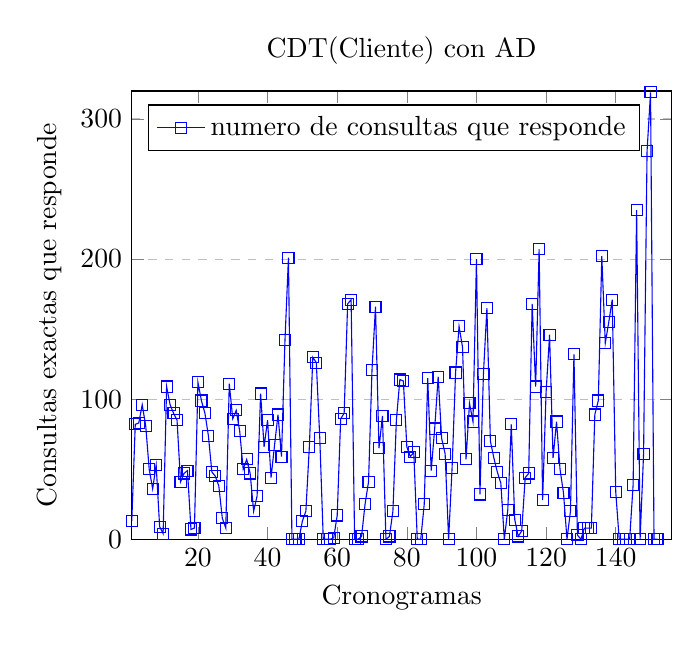
\begin{tikzpicture}
\begin{axis}[
    %CDT = carga de trabajo
    %AEPxT = Algoritmo DETERMINISTA
    title={CDT(Cliente) con AD},
    xlabel={Cronogramas},
    ylabel={Consultas exactas que responde},
    xmin=1, xmax=156,
    ymin=0, ymax=320,
    xtick={},
    ytick={},
    legend pos=north west,
    ymajorgrids=true,
    grid style=dashed,
]

\addplot[
    color=blue,
    mark=square,
    ]
    coordinates {
   %CARGA DE TRABAJO CLIENTE
   (1,13)
(2,82)
(3,83)
(4,96)
(5,81)
(6,50)
(7,36)
(8,53)
(9,9)
(10,4)
(11,109)
(12,96)
(13,90)
(14,85)
(15,41)
(16,47)
(17,49)
(18,7)
(19,8)
(20,112)
(21,99)
(22,90)
(23,74)
(24,48)
(25,45)
(26,38)
(27,15)
(28,8)
(29,111)
(30,86)
(31,92)
(32,77)
(33,50)
(34,57)
(35,47)
(36,20)
(37,31)
(38,104)
(39,66)
(40,85)
(41,44)
(42,67)
(43,89)
(44,59)
(45,142)
(46,201)
(47,0)
(48,0)
(49,0)
(50,13)
(51,20)
(52,66)
(53,130)
(54,126)
(55,72)
(56,0)
(57,0)
(58,0)
(59,1)
(60,17)
(61,86)
(62,90)
(63,168)
(64,171)
(65,0)
(66,0)
(67,2)
(68,25)
(69,41)
(70,121)
(71,166)
(72,65)
(73,88)
(74,0)
(75,2)
(76,20)
(77,85)
(78,114)
(79,113)
(80,66)
(81,59)
(82,62)
(83,0)
(84,0)
(85,25)
(86,115)
(87,49)
(88,79)
(89,116)
(90,72)
(91,61)
(92,0)
(93,51)
(94,119)
(95,152)
(96,137)
(97,57)
(98,97)
(99,84)
(100,200)
(101,32)
(102,118)
(103,165)
(104,70)
(105,58)
(106,48)
(107,40)
(108,0)
(109,21)
(110,82)
(111,14)
(112,2)
(113,6)
(114,44)
(115,47)
(116,168)
(117,109)
(118,207)
(119,28)
(120,105)
(121,146)
(122,58)
(123,84)
(124,50)
(125,33)
(126,0)
(127,20)
(128,132)
(129,3)
(130,0)
(131,8)
(132,8)
(133,8)
(134,89)
(135,99)
(136,202)
(137,140)
(138,155)
(139,171)
(140,34)
(141,0)
(142,0)
(143,0)
(144,0)
(145,39)
(146,235)
(147,0)
(148,61)
(149,277)
(150,319)
(151,0)
(152,0)
    };
    \legend{numero de consultas que responde}

\end{axis}
\end{tikzpicture}